\documentclass[12pt,a4paper,leqno]{report}

\usepackage[T1]{fontenc}
\usepackage[english]{babel}
\usepackage{amsthm}
\usepackage{amsfonts}
\usepackage{amsmath}
\usepackage{amssymb}
\usepackage{tikz}
\usepackage{listings}

\newcommand{\R}{\mathbb{R}}
\newcommand{\C}{\mathbb{C}}
\newcommand{\Q}{\mathbb{Q}}
\newcommand{\N}{\mathbb{N}}
\newcommand{\No}{\mathbb{N}_0}
\newcommand{\Z}{\mathbb{Z}}
\newcommand{\diam}{\operatorname{diam}}

\theoremstyle{plain}
\newtheorem{equa}[equation]{Equation}
\newtheorem{lem}[equation]{Lemma}
\newtheorem{prop}[equation]{Proposition}
\newtheorem{cor}[equation]{Corollary}

\theoremstyle{definition}
\newtheorem{defi}[equation]{definition}
\newtheorem{conj}[equation]{Conjecture}
\newtheorem{example}[equation]{Example}
\theoremstyle{remark}
\newtheorem{note}[equation]{Note}

\pagestyle{plain}
\makeatletter
\renewcommand{\@seccntformat}[1]{}
\makeatother
\setcounter{page}{1}
\addtolength{\hoffset}{-1.15cm}
\addtolength{\textwidth}{2.3cm}
\addtolength{\voffset}{0.45cm}
\addtolength{\textheight}{-0.9cm}

\graphicspath{ {./figures/} }

\title{Big Data - Lessons Learned}
\author{Tuomo Kareoja}
\date{\today}

\begin{document}

\maketitle

\newpage

\section{Model Creationg}

\subsection{Chosen Model and Features}

Random forest model was chosen for creating the final predictions for both iPhones
and Samsung Galaxy phones. This model offered the best cross-validation metrics
with least variation, so we can think that on top of being accurate the model
is also quite stable to extreme values in the training data.

For all tested models (gradient boosting, k-nearest neighbors and random forest) same kind of
feature selection process was used. Before even starting the analysis we manually dropped
all features related to HTC phones. These features had in the initial testing some predictive
power for the Samsung Galaxy Sentiment, but it was thought that this was because
HTC used to manufacture the Google Pixel phones where that serve as a testbed for the latest
Android operation system versions. Supporting this conclusion was that HTC features were
highly correlated with Android operations system features, meaning that this where very
often mentioned in the the same website. HTC does no longer manufacture Pixel
phones so, we thought that this connection was not stabile over time and newer articles
could be mislabeled if we kept these features in our models.

After dropping the HTC features, rest of the feature selection was done automatically
with recursive feature elimination. In this method the models were run multiple times with
different parts of the data (rows) while an algorithm tries to drop variables up to the point
where model predictive power started to decline.

Chosen features for the random forest iPhone model were:

\begin{itemize}
    \item iphone
    \item samsunggalaxy
    \item ios
    \item googleandroid
    \item iphonecampos
    \item samsungcampos
    \item iphonecamneg
    \item samsungcamneg
    \item iphonecamunc
    \item samsungcamunc
    \item iphonedispos
    \item samsungdispos
    \item iphonedisneg
    \item samsungdisneg
    \item iphonedisunc
    \item samsungdisunc
    \item iphoneperpos
    \item samsungperpos
    \item iphoneperneg
    \item samsungperneg
    \item iphoneperunc
    \item samsungperunc
    \item googleperpos
    \item iosperunc
    \item googleperunc
\end{itemize}

For Galaxy model we ended up with the same features except without googleperunc
(number of statements about Android operating system with unclear sentiment).

Below are the crossvalidation metrics of the tested models.
This cross-validation was done with the full dataset, but the initial model selection and hyperparameter tuning was done with a separated train
and test set. As the models and features were set in stone already by this previous process with holdout data, we did not see any reason to create a separate
test set for the model comparison.

These are just the graphs for the iPhone models as the graphs for Galaxy models looks almost identical so I
did not think it useful to include them.

{
    \centering
    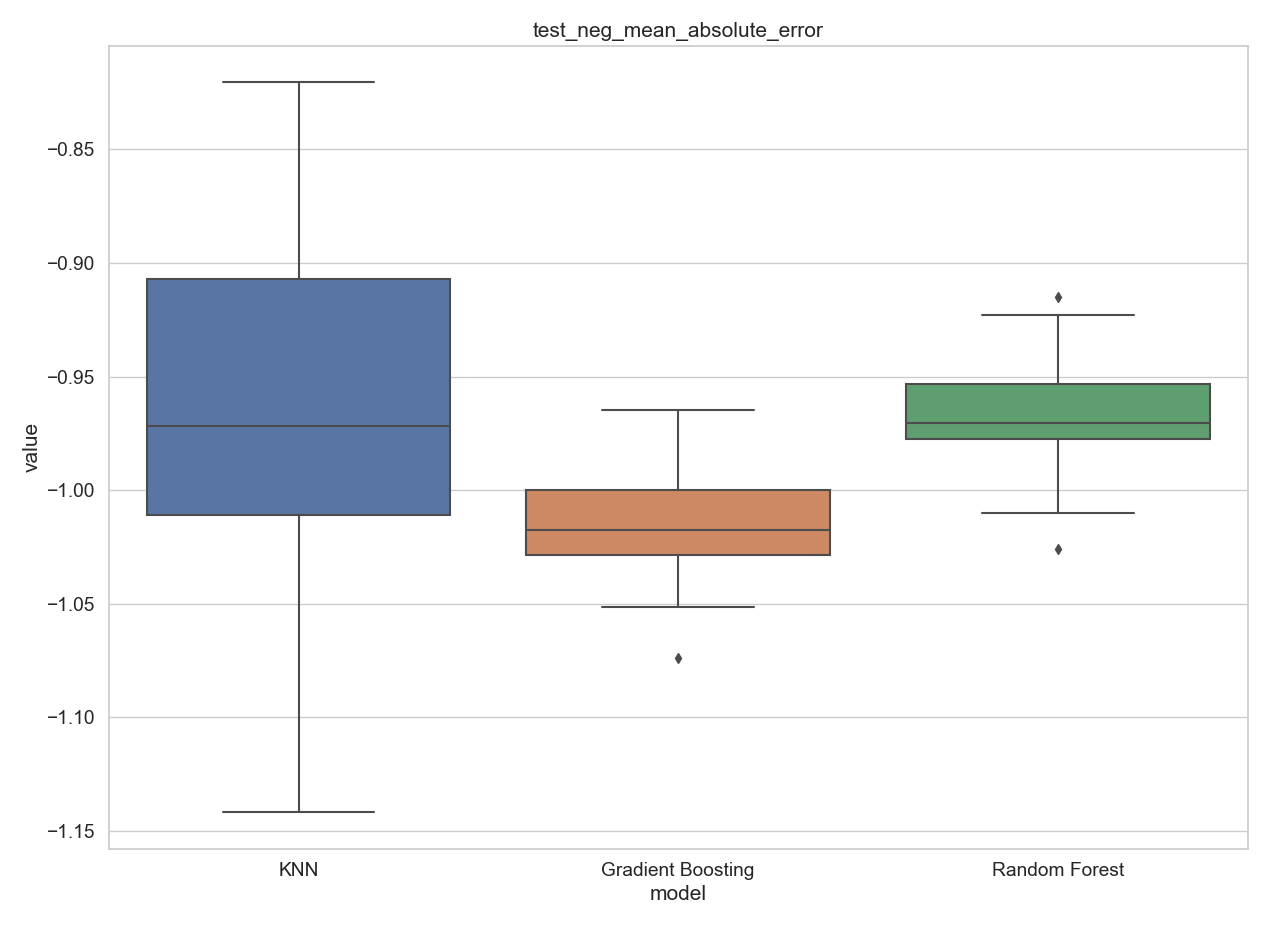
\includegraphics[width=\textwidth,height=\textheight,keepaspectratio]{model_comparison_iphone_test_neg_mean_absolute_error.png}
    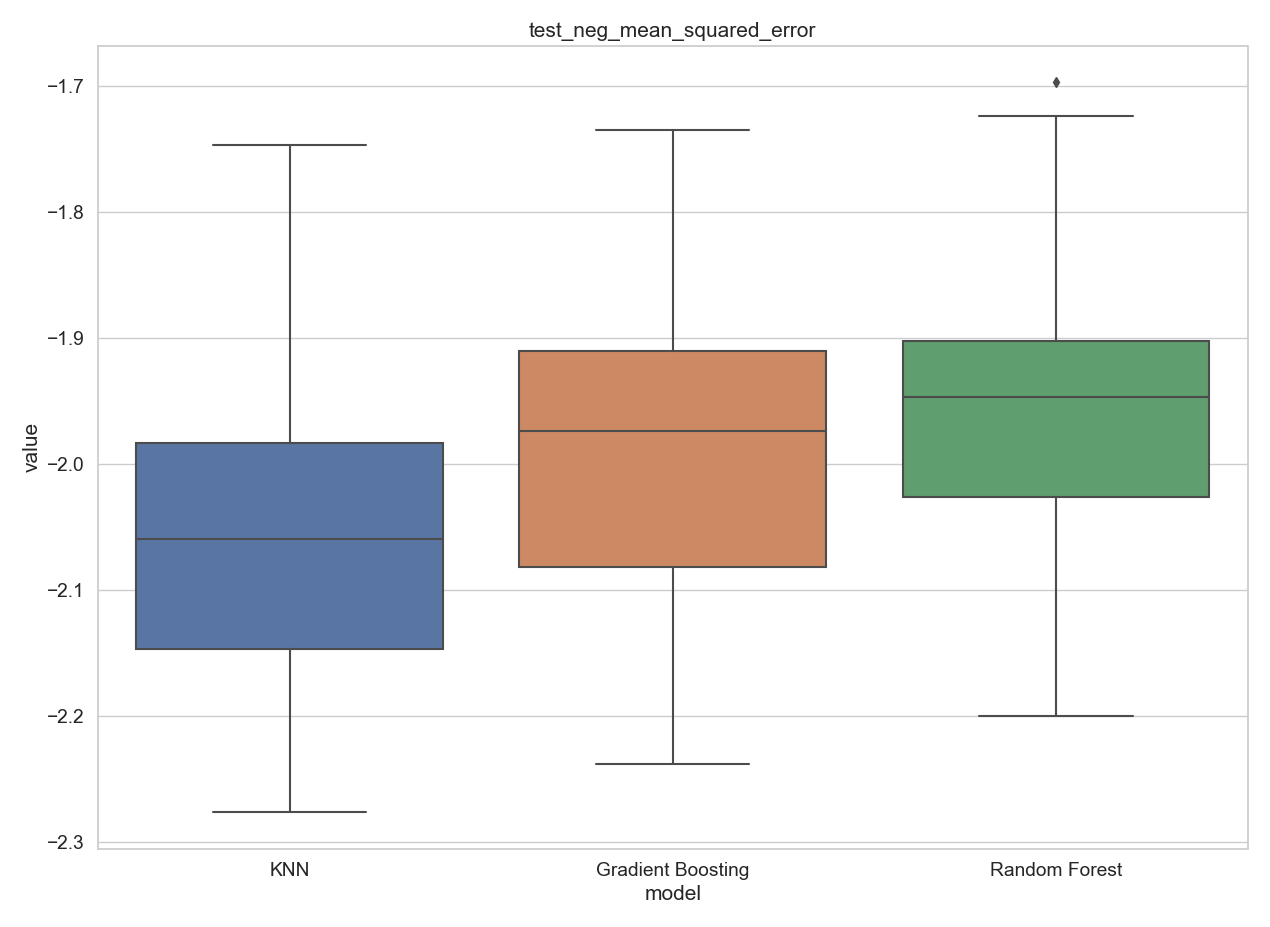
\includegraphics[width=\textwidth,height=\textheight,keepaspectratio]{model_comparison_iphone_test_neg_mean_squared_error.png}
    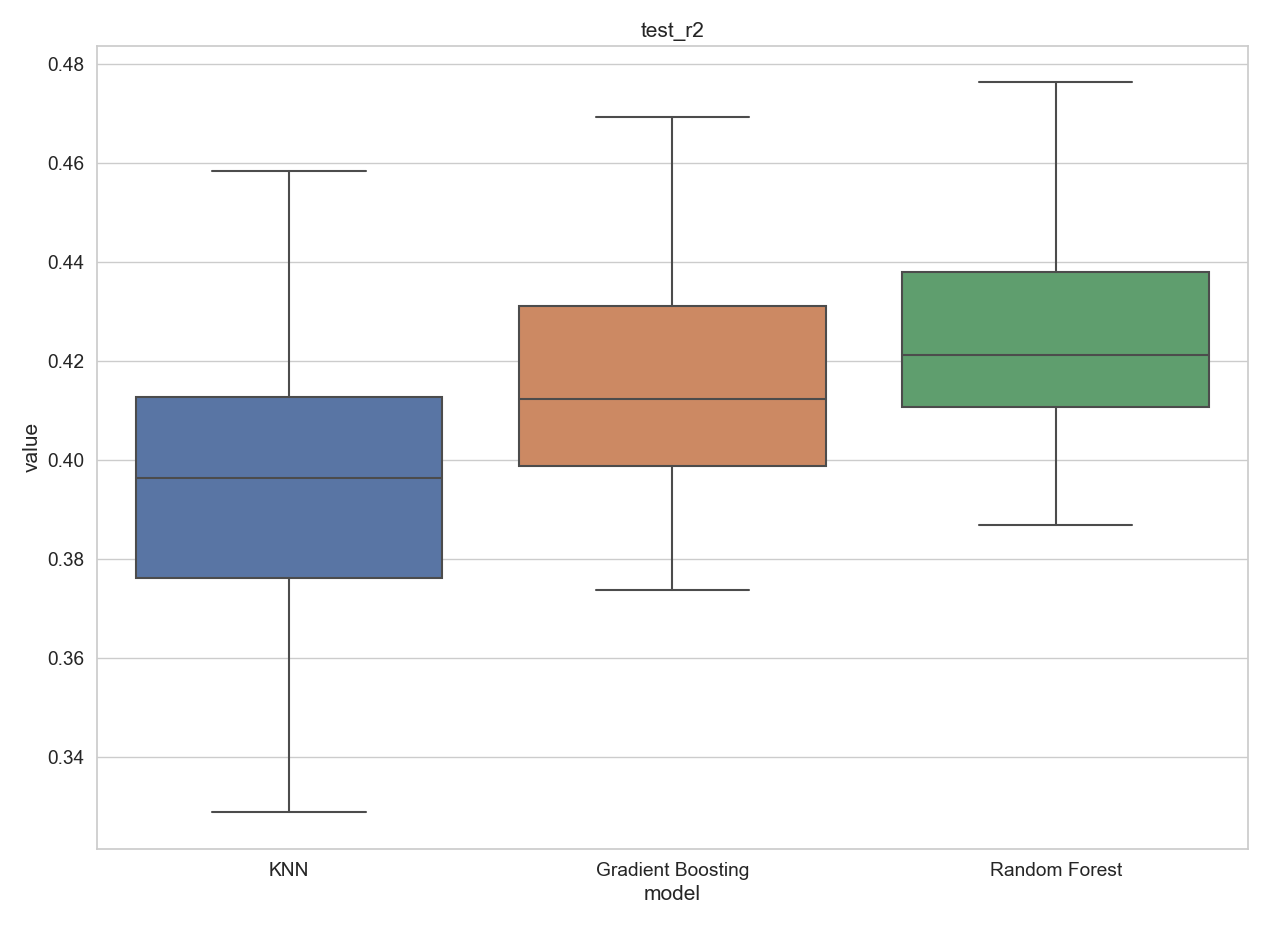
\includegraphics[width=\textwidth,height=\textheight,keepaspectratio]{model_comparison_iphone_test_r2.png}
    \par
}

\section{Problems}

\subsection{Very Hard to Know are What the Results Mean When You don't Trust the Training Data}

The training data had the weird quality that also sites that did not include mentions of
the phones were labeled with sentiments. First I thought that this was because missing values
were also labeled as zero, but this was not the case as the sites not mentioning the phones
had a wide spectrum of sentiments. This was especially true for Galaxy phones where almost
all websites had no mentions of the phone. When I looked at the correlation between the
sentiment values (these were coded for the same websites), it was clear that the sentiment
values were not created separately, but that maybe the galaxy values were created from iphone
values by some adding some slight variation. How could it otherwise be possible that
the sentiment for the Samsung Galaxy phone is always the same or one point higher (more positive)
than iPhone in the same websites? Below are two graphs demonstrating these problems.

{
    \centering
    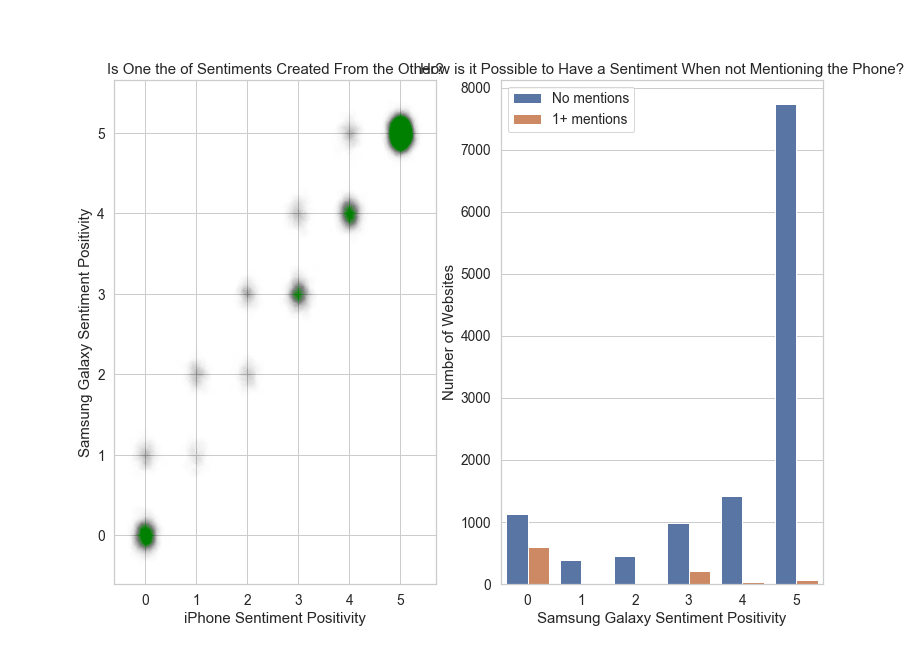
\includegraphics[width=\textwidth,height=\textheight,keepaspectratio]{training_data_problems.png}
    \par
}

Because almost all the variation in sentiment for Samsung Galaxy comes from
sites that do not mention the phone (see right graph on top), I think that these values are not
real and were deduced from iphone sentiment by some random method. This leads me to conclude
that the sentiment for Galaxy Phones cannot be trusted.

\subsection{Web Crawling Hits too Many Random Websites}

Crawling the random websites works, but it was unclear what kind of sites we are
actually trying to find and how to avoid weird sites that have mentions of the
phones for some search engine optimization reason or some other weird quirk.

Below are wordclouds for the urls of the websites that contain over 10 mentions
of the phones in questions. The Galaxy graph seems smaller because it had problems
actually finding that enough suitable sites.

Words for iPhone websites seem actually quite sensible, with words like iphone, review, best,
phone and so on, but there also really weird ones. The two most common words are sidehustehq
and danhostel. The first is a site giving advice on how to make money from different
side jobs, e.g. making simple IOS apps for iPhone. Danhostel is danish hotel chain
that has an app for iPhone. It is not clear if these were the kinds of sites that we
were looking for.

The case with Galaxy Phone sites is more clear: these where not the sites we were looking for.
Different mentions of Texas counties and countries come from the same website
http://brazoriacountytexas.tk/ that is just a hyperlink jungle without any real contnent,
probably created to fool web crawlers like us.

{
    \centering
    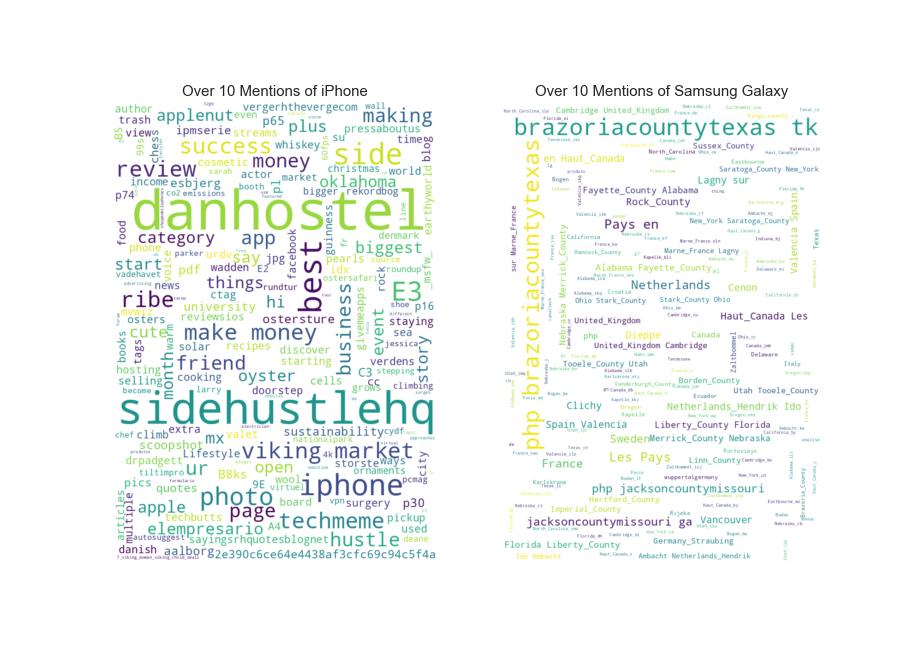
\includegraphics[width=\textwidth,height=\textheight,keepaspectratio]{wordclouds_for_sites_with_lots_of_mentions.png}
    \par
}

\section{What Should be Changed in Our Data Science Process?}

\subsection{Data Creation Should be Documented Better}

The biggest problem in the project was the where the training data came
from and could it be trusted was highly questionable. It was mentioned that
the data was manually labeled, but if this was the case what was the
scoring criteria. On the other hand, if the labeling was done by an algorithm,
then the code that created the labels should be shared. Also
why did the training set not include URLs for the coded websites?

As was mentioned previously, the training must be in some erroneous, but
it is hard to pinpoint where did the error come from without this kind
of documentation.

\subsection{Collaboration Between Data Scientists Should be a Two Way Street}

The training data was provided by somebody else with just a few words
documentation and contact information. The features and the scripts for calculating
them were also created by somebody else. This led to the situation
where I had to rely on my analysis on parts who's function was not completely
clear to me, and where I could not make corrections when problems were found
(especially with the training data). This kind of collaboration is a very
bad idea, because we separate parts of the analysis to multiple people and
these people are not responsible for the project outcome, it can lead to
situation where they pass subpar or erroneous code or data and then just
jump to the next project, leaving somebody else to have to deal with the consequences.

Everybody contributing to the project should in future be available for changes
and corrections for the whole duration of the project and share the responsibility
of the outcome.

\end{document}
